\section*{Supporting Information Captions}
% Supporting graphics remain visible in this drafting version.
\setcounter{figure}{0}
\renewcommand{\thefigure}{S\arabic{figure}}
\renewcommand{\theHfigure}{supp.\arabic{figure}}
\captionsetup[figure]{labelformat=plossupport}

Supporting Table~S1 is the copied regulatory-enrichment workbook
\path{figures/Fig3_Hyper_table.xlsx}. Supporting Table~S2 is the copied
motif workbook \path{figures/Fig6_Motif_table.xlsx}. They remain native
spreadsheets and are not rendered as LaTeX figures. Table~S2 has updated numeric
cells but inherited manual biological annotations; its ``MR-only'' title
should be reviewed because the underlying foregrounds are method-specific.
\TODO{Convert selected supporting-table content to manuscript tables after
review; do not treat inherited annotation text as independently verified.}

\noindent\textbf{S1 Table. Regulatory-reference enrichment workbook.}
\TODO{Finalize the supporting-table caption and file format after review of
the existing workbook; no table content has been revised.}

\noindent\textbf{S2 Table. Motif enrichment workbook.}
\TODO{Finalize the supporting-table caption after review of the inherited
annotations and foreground description noted above.}

\noindent\textbf{S1 Checklist. STROBE-MR reporting checklist (pending).}
\TODO{Prepare the completed reporting checklist with manuscript page numbers
and relevant text. This label reserves a supporting item; no completed
checklist is currently supplied.}

\begin{figure}[p]
\centering
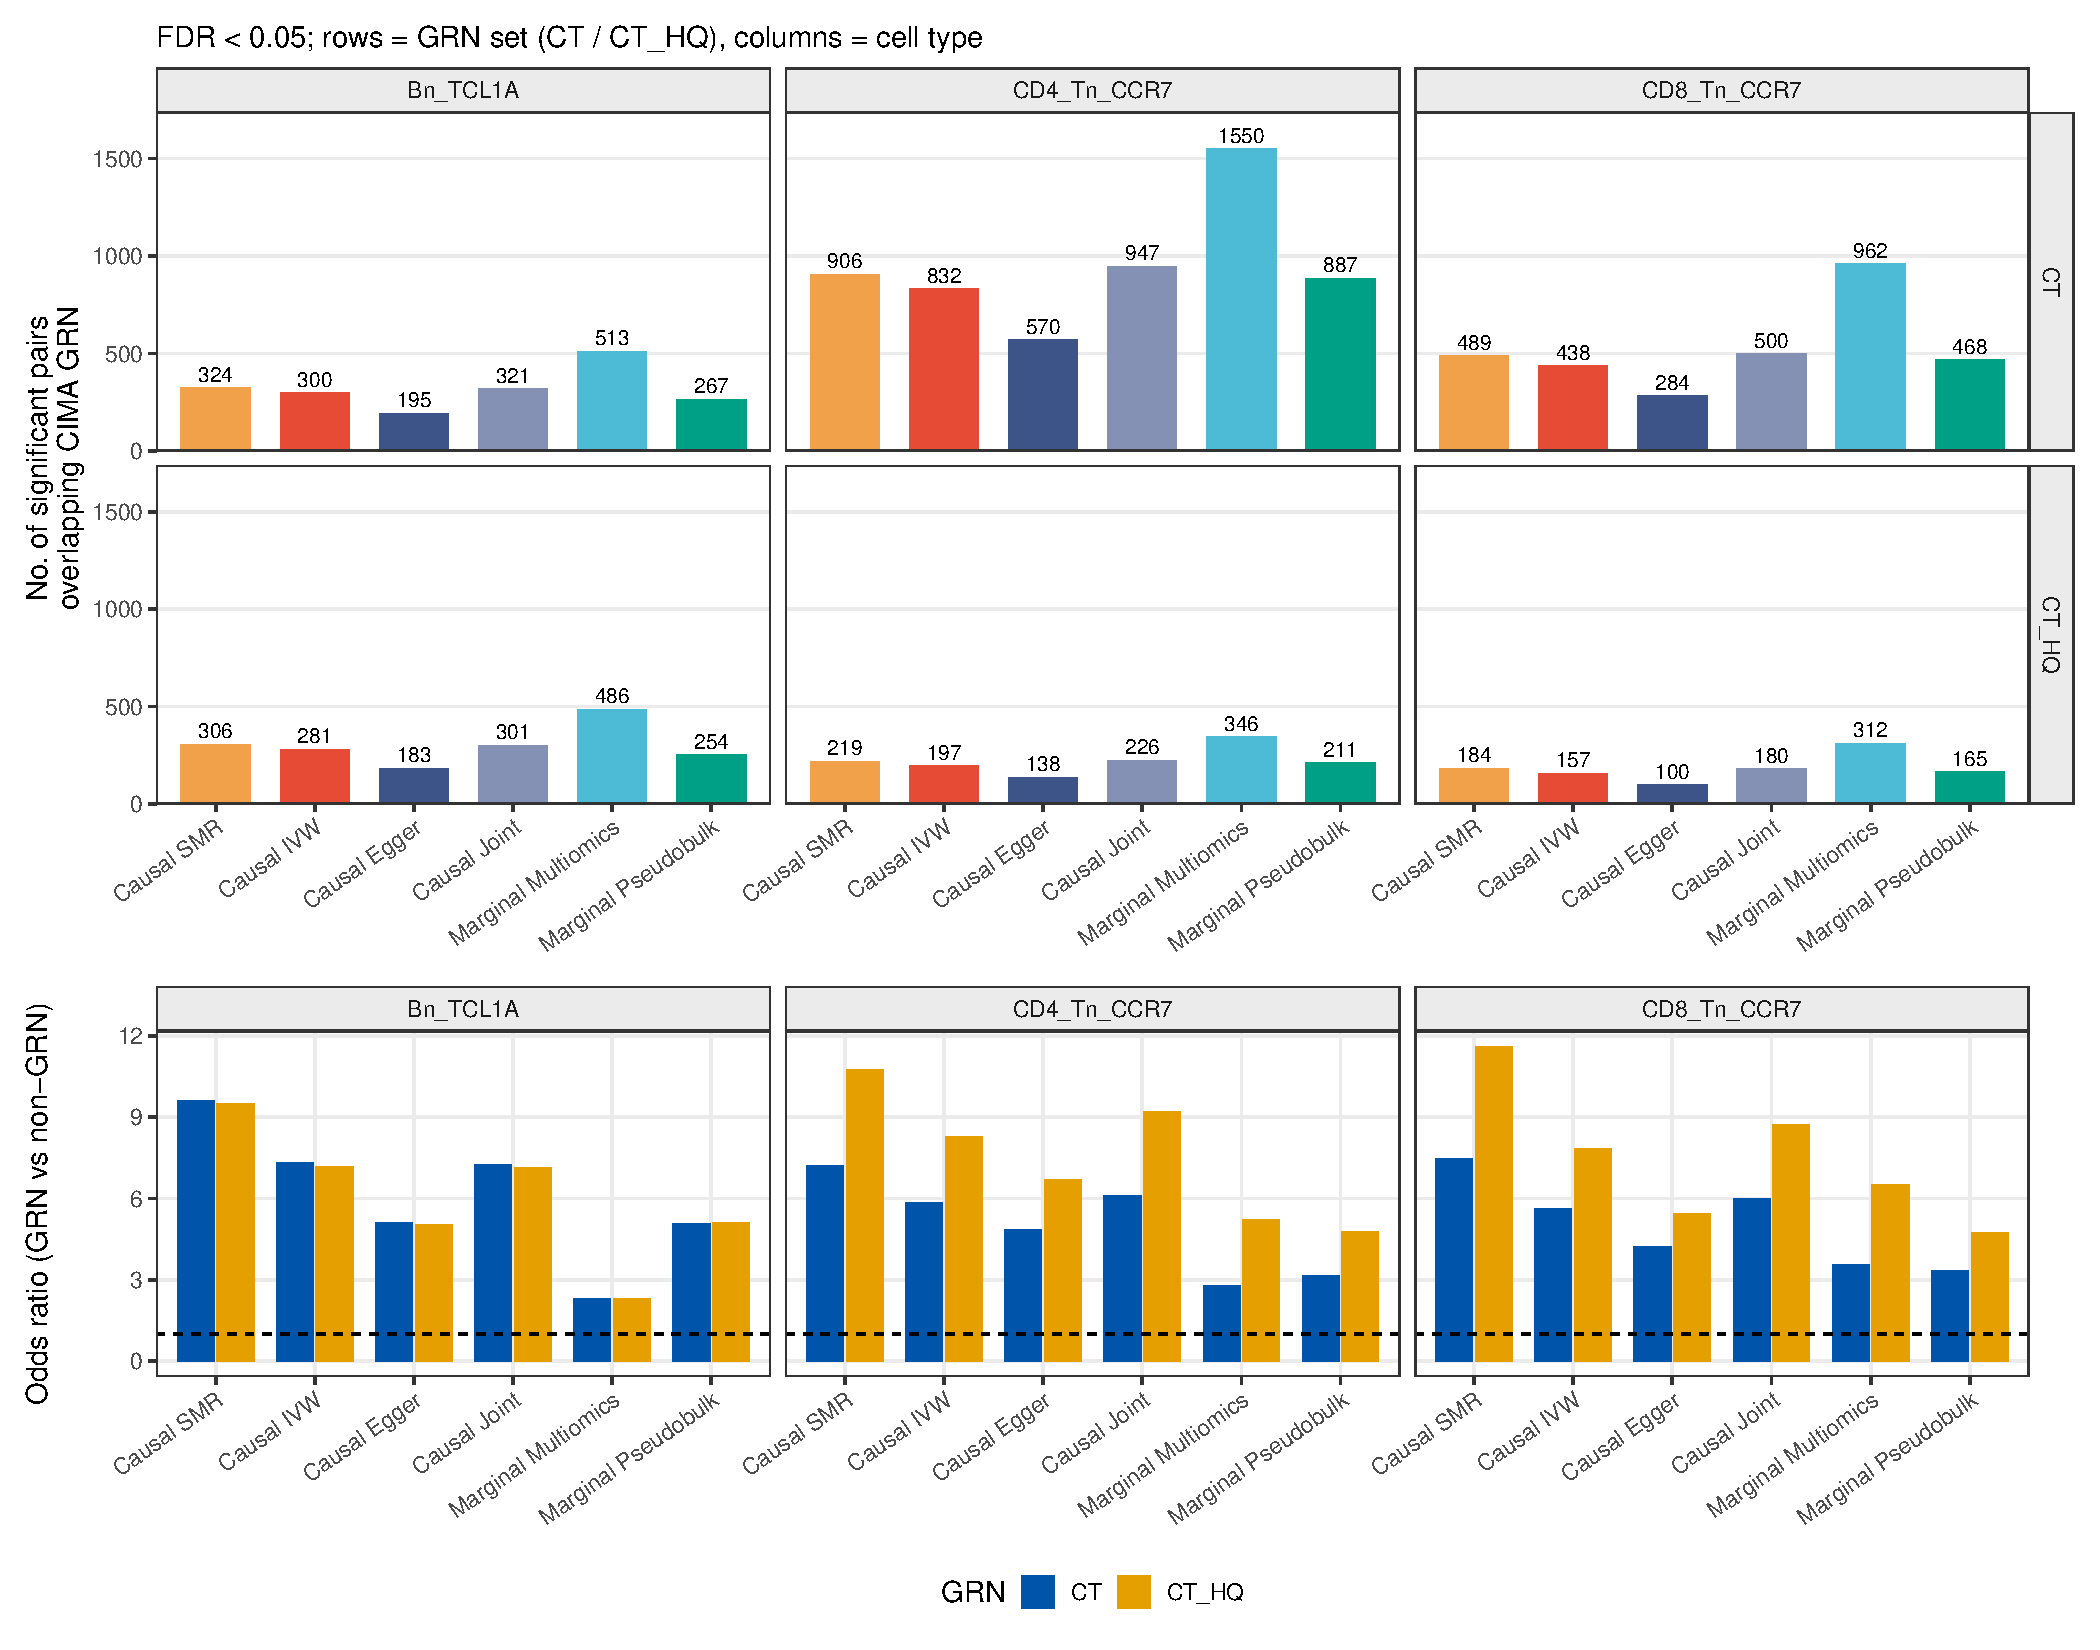
\includegraphics[page=1,width=\linewidth,height=0.78\textheight,keepaspectratio]{Fig7_GRN.pdf}
\caption{Within-CIMA GRN corroboration. Top panels show significant-pair
overlap counts at \(\q<0.05\) for cell-type-active networks (CT) and their
lineage high-quality subset (CT\_HQ). Bottom panels show Fisher odds ratios
relative to non-GRN tested pairs. This unchanged one-page figure is the latest
available GRN artifact in the older figure directory.}
\label{fig:supp-grn}
\end{figure}

\begin{figure}[p]
\centering
\includegraphics[page=2,width=\linewidth,height=0.70\textheight,keepaspectratio]{Fig9_GO_GSEA.pdf}
\caption{Conventional GO BP GSEA for the 4,509 combined MR-only target genes.
The five terms with smallest conventional GSEA p-values are shown as
\(-\log_{10}\) BH-adjusted p-values; the dashed line marks adjusted \(p=0.1\).
This is unchanged source page 2. Pages 1 and 3 of the copied PDF contain
per-group conventional-p and empirical-p displays, respectively, and are not
silently combined with this conventional comparison.}
\label{fig:supp-go}
\end{figure}

\begin{figure}[p]
\centering
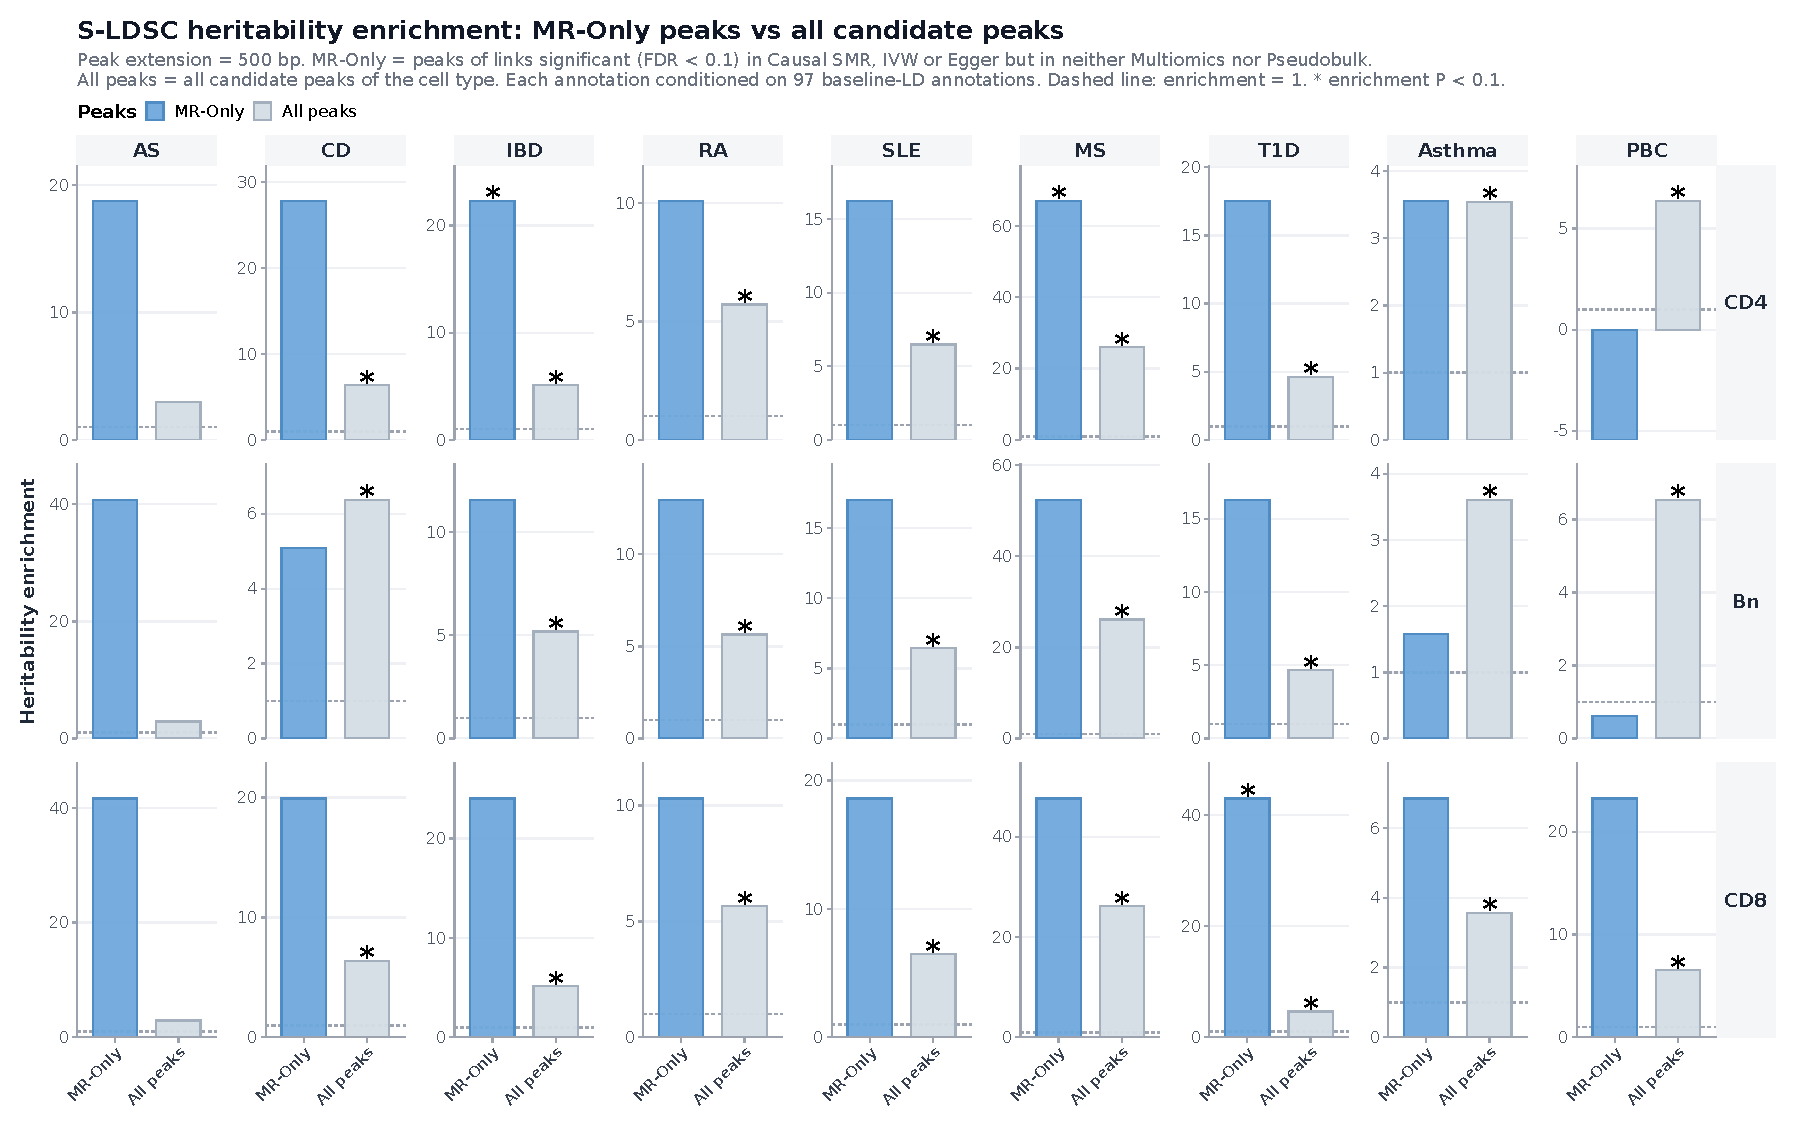
\includegraphics[page=1,width=\linewidth]{Fig5_SLDSC.pdf}
\caption{Cell-type-specific S-LDSC enrichment. The unchanged source page 1
compares MROnly and all-candidate-peak annotations for CD4, Bn, and CD8, with
the definition and raw-p asterisk convention of Figure~\ref{fig:sldsc}.
Axis scales differ between panels.}
\label{fig:supp-sldsc}
\end{figure}

\begin{figure}[p]
\centering
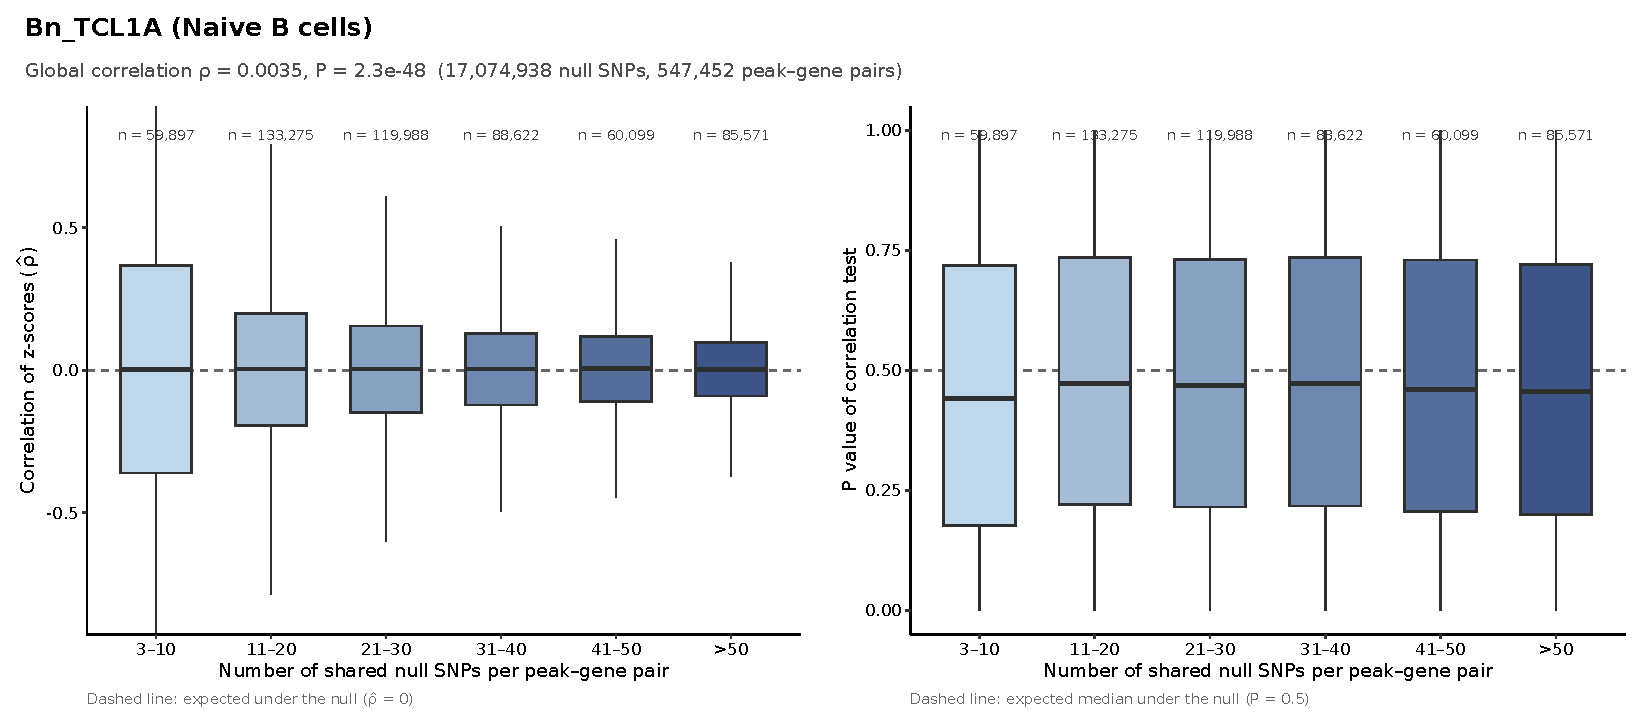
\includegraphics[page=1,width=\linewidth]{Sup1_OneSampleMR.pdf}
\caption{Null-SNP diagnostic in Bn. Pair-level correlations of caQTL and
eQTL z-scores, and their correlation-test p-values, are grouped by the number
of shared pruned null SNPs. The displayed global summary pools SNP--pair
observations; repeated variants may contribute to multiple pairs. This is
unchanged source page 1, with CD4 and CD8 retained as pages 2 and 3 in the
copied PDF. The diagnostic does not itself establish MR calibration.}
\label{fig:supp-qc}
\end{figure}
\FloatBarrier
